% !TeX root = ../../book.tex
\section{真理与证明}\label{sec:section1.1}

你怎么知道一件事是真是假?比如,上学时老师告诉你三角形的内角和为 $180$ 度,但你怎么\emph{知道}这是真的呢?万一你遇到一个从来没有学过基础几何的外星人呢?你如何\emph{说服}他/她/它相信这是真的呢?从某种程度上说,这就是数学:设计新的陈述,以某种方式确定它们是真是假,并向其他人(也可能是外星人)解释这些发现。不幸的是,似乎很多人认为数学家成天做的就是把大数乘在一起;但事实上,数学是一门更具创造性和写作基础的学科,而不是人们普遍认为的复杂算术。本书的目标之一就是让你相信这一事实,但这不是主要目标。本书的主要目标是向你揭示数学思维、解决问题和给出证明的真正意义,并教你如何完成这些事情,以及它们是多么的有趣!

顺便一提,你可能好奇``某事为真意味着什么''?要想全面讨论这个问题需要深入到哲学、心理学、或许还有语言学层面,我们不想太过深入其中。然而就数学而言,其主要思想是:\textbf{只有我们能够}\emph{证明}\textbf{某事}\emph{永远}\textbf{为真它才为真}。我们知道 $1+1=2$ 永远为真。无论是黑夜还是白天,该等式永远成立。(不过,你有没有想过如何证明这一事实?实际上证明这个问题非常困难!有本名为\emph{《数学原理》}的书从``第一性原理''出发,经过很多很多页论证才得出 $1+1=2$!)这或许与其他科学完全不同。如果我们进行 $10$ 次物理实验并且观测到相同的结果,我们是否可以断定它会\emph{永远}发生?要是我们做一百万次实验会怎样?十亿次呢?我们在什么时点真正给出了\emph{证明}?在数学上,反复实验不是可行的证明!我们需要找到一个论证来说明为什么这种现象总会发生。举个例子,数学中有个著名的未解难题叫\href{https://baike.baidu.com/item/哥德巴赫猜想/72364}{哥德巴赫猜想}。目前还不知道其是否正确,尽管我们已经通过计算机模拟验证到大约 $10^{18}$ 都是正确的。$10^{18}$ 是个\emph{巨大的}天文数字,但仍不足以证明猜想是\textbf{真}是\textbf{假}。你看到差别了吗?数学家喜欢\emph{证明}事实,而不是用一堆值去检验,检验值只要不是\emph{全部}就\emph{不能}构成证明。

\subsection{三角迷思}\label{sec:section1.1.1}

通过讨论我们希望证明完成什么以及为什么我们如此关心证明,我们引入了\textbf{证明}的概念。那么,你可能会问如何\emph{定义}证明。这实际上是一个很难解释的思想!为了接近这一思想,我们将给出几个不同的数学论证。希望你都阅读一下,并思考它们是否具有说服力。它们\emph{证明}了什么?它们正确吗?它们是可以理解的吗?它们让你感觉如何?先自己思考形成一些观点,然后再阅读我们的讨论。

我们给出的数学论证都与三角形有关。具体来说,都涉及\textbf{毕达哥拉斯定理}。

\begin{theorem}[毕达哥拉斯定理] \label{thm:pythagorean}
    如果直角三角形两直角边长为 $a,b$,斜边长为 $c$,则它们 $a^2+b^2=c^2$。
\end{theorem}

\begin{center}
    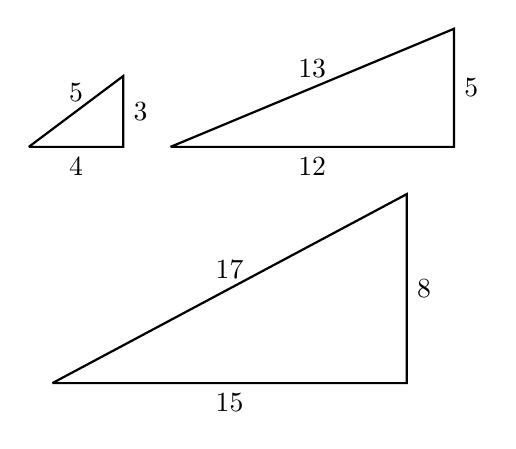
\begin{tikzpicture}[thick, scale=0.30]
        \draw (0,0) -- (4,0) node[midway,below]{$4$}
        -- (4,3) node[midway,right]{$3$}
        -- (0,0) node[midway,above]{$5$};
        \draw (6,0) -- (18,0) node[midway,below]{$12$}
        -- (18,5) node[midway,right]{$5$}
        -- (6,0) node[midway,above]{$13$};
        \draw (1,-10) -- (16,-10) node[midway,below]{$15$}
        -- (16,-2) node[midway,right]{$8$}
        -- (1,-10) node[midway,above]{$17$};
    \end{tikzpicture}
\end{center}

我们是怎么知道的呢?这是一个非常有用的事实,你可能在数学课上(或者生活中不经意地)用过很多次。你有没有思考过为什么这是真的?你会如何向持怀疑态度的朋友解释呢?这就是\textbf{数学证明}试图完成的:对事实的清晰简洁的解释。要求证明背后的原因也十分有意义,它具有两重含义:确信我们认为是真的事情确实真的,并且要使用时不必每次都其进行解释。在(令人满意地)证明毕达哥拉斯定理之后,我们只需在相关情况出现时通过名字引用该定理即可;我们已经证明过了,所以无需再次证明。

那么,究竟什么构成了证明?怎么知道解释是否足够清晰和简洁?一般来说,回答这个问题相当困难,这也是为什么数学既可以被视为科学,也可以被视为艺术的部分原因。没错,我们处理的都是冰冷艰涩的事实,但能够对这些事实进行推理并向他人以令人满意的形式解释清楚,这本身就是一种艺术。

\subsubsection*{``证明''范例}

让我们一起看几个``证明''的例子,看看它们是否足够好。(我们现在先说``证明'',稍后为其下更精确的定义。)这里是第一个:

\begin{proofs}{``证明'' 1.}
    画一个边长为 $a+b$ 的正方形。在这个正方形里画 $4$ 个相同的直角三角形,这 $4$ 个直角三角形在大正方形的内部组成一个边长为 $c$ 的正方形。

    \begin{center}
        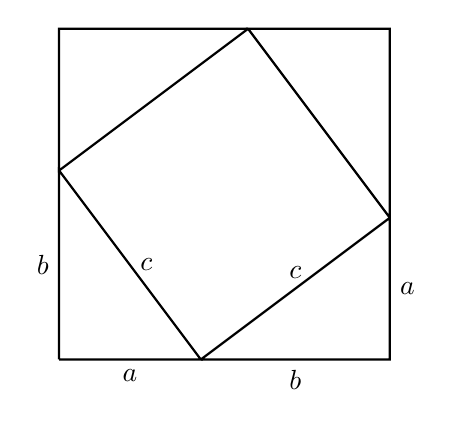
\begin{tikzpicture}[thick, scale=0.6]
            \draw (0,0) -- (3,0) node[midway,below]{$a$}
            -- (0,4) node[midway,right]{$c$}
            -- (0,0) node[midway,left]{$b$};
            \draw (3,0) -- (7,0) node[midway,below]{$b$}
            -- (7,3) node[midway,right]{$a$}
            -- (3,0) node[midway,above]{$c$};
            \draw (7,3) -- (7,7)
            -- (4,7)
            -- (7,3);
            \draw (4,7) -- (0,7)
            -- (0,4)
            -- (4,7);
        \end{tikzpicture}
    \end{center}

    大正方形的面积可以用两种方式表示:应用正方形的面积公式,或者把小正方形和四个三角形的面积加起来。因此,下面这个等式一定成立。
    \[(a+b)^2=c^2+4\cdot\frac{ab}{2}=c^2+2ab\] 
    将左边表达式展开,然后两边同时消掉同类项可得 
    \[a^2+\cancel{2ab}+b^2=c^2+\cancel{2ab}\] 
    所以,$a^2+b^2=c^2$ 成立。
\end{proofs}

上面的证明能说服你吗?每一步都合理吗?可能你现在还不确定,所以让我们看一下此定理的另外一种``证明''。

\begin{proofs}{``证明'' 2.}
    假设毕达哥拉斯定义成立,绘制直角三角形,并过直角对应的顶点做高。如下图所示标记点和边长:
    \begin{center}
        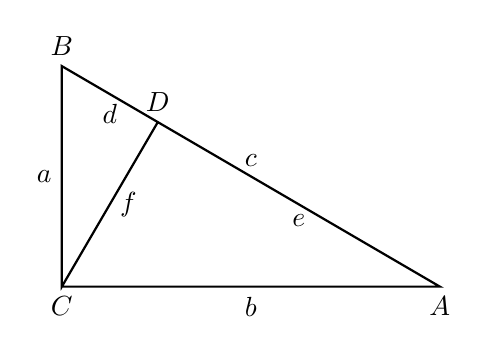
\begin{tikzpicture}[thick, scale=0.8]
            \coordinate (C) at (0,0);
            \coordinate (A) at (6,0);
            \coordinate (B) at (0,3.5);
            \coordinate (D) at (1.523316, 2.611399);
            \draw (C) node[anchor=north]{$C$}
            -- (A) node[anchor=north]{$A$} node[midway,below]{$b$} 
            -- (B) node[anchor=south]{$B$} node[midway,above]{$c$}
            -- (C) node[midway,left]{$a$}
            -- (D) node[anchor=south]{$D$} node[midway,right]{$f$}
            -- (A) node[midway,below]{$e$} 
            -- (D)
            -- (B) node[midway,below]{$d$};
            \rightAngle{B}{D}{C}{0.3};
        \end{tikzpicture}
    \end{center}
    因为毕达哥拉斯定理成立,所以我们可以将其应用到图中的三个直角三角形中,即三角形 $ABC, BCD, ACD$。(定义 $e = c-d$)可得
    \begin{align*}
        a^2 &= d^2 + f^2 \\
        b^2 &= f^2 + e^2 \\
        c^2 &= a^2 + b^2
    \end{align*}
    将前两个方程相加再用第三个方程替换,可得
    \[c^2 = d^2 + e^2 +2f^2\]
    请注意,角 $\angle ABC$ 和 $\angle ACD$ 相等,因为它们都与角 $\angle CAB$ 互补,因此我们知道三角形 $\triangle CDB$ 和 $\triangle ADC$ 是相似三角形。(这里假设你对平面有一定了解。)由此可得 $\frac{e}{f} = \frac{f}{d}$,因此 $f^2 = ed$。我们可以将其带入上面的公式替换 $f^2$,结果如下:
    \[c^2 = d^2+e^2+2de = (d+e)^2\]
    两边同时开方(已知 $c,d,e$ 都是正数)可得 $c = d+e$,根据边长 $d$ 和 $e$ 的定义,这显然成立。因此,假设毕达哥拉斯定理成立是正确的。
\end{proofs}

这个证明怎么样?有说服力吗?清楚吗?在我们确定什么构成``正确的''或``良好的''证明之前,让我们再检验一个``证明''。

\begin{proofs}{``证明'' 3.}
    观察下图
    \begin{center}
        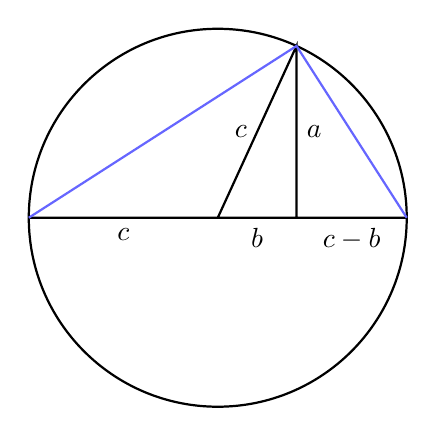
\begin{tikzpicture}[thick, scale=0.4]
            \coordinate (O) at (0,0);
            \coordinate (A) at (-6,0);
            \coordinate (B) at (6,0);
            \coordinate (C) at (2.5,0);
            \coordinate (D) at (2.5,5.45435);
            \draw (O) circle (6);
            \draw (A) -- (O) node[midway,below]{$c$}
            -- (C) node[midway,below]{$b$}
            -- (B) node[midway,below]{$c-b$}
            -- (C)
            -- (D) node[midway,right]{$a$}
            -- (O) node[midway,left]{$c$};
            \draw[color=blue!60] (A) -- (D) -- (B);
            \rightAngle{B}{C}{D}{0.6};
        \end{tikzpicture}
    \end{center}  
    易得 $\frac{a}{b+c} = \frac{c-b}{a}$,因此 $a^2 + b^2 = c^2$。
\end{proofs}

这个证明对你来合理吗?最后,还有一个需要思考的``证明''。

\begin{proofs}{``证明'' 4.}
    毕达哥拉斯定理一定成立,否则我的老师就一直在骗我。
\end{proofs} 

\subsubsection*{讨论}

在继续阅读之前,我们鼓励你先思考一下这四个``证明'',甚至与同学或朋友讨论一下。你认为什么构成``正确''的证明?清晰性和易读性重要吗?它会影响证明的``正确性''吗?

从历史的角度来看,数学证明的撰写已经发展了多年,并且对于什么构成``正确''的证明存在良好的普遍共识:

\begin{itemize}
    \item 从数学角度来说,证明中的每一\emph{步}、每一个逻辑推论和主张都是\emph{有效的},这一点很重要。
    \item 同样重要的是,证明撰写者必须(合理地)明确为什么某个陈述来自先前的工作或外部知识。
\end{itemize}

\emph{真理}的这些要求的好处在于,一旦数学已经建立起来,我们就可以通读一个论证并验证每个主张是\textbf{对}还是\textbf{错}。难以定义的是清晰的写作。在某种程度上,这很像最高法院法官波特·斯图尔特(Justice Potter Stewart)对淫秽的著名定义:``当我看到它时,我就知道''。

让我们对给出的四个论证进行比较,评估它们的清晰性和正确性:

\textbf{清晰性:}

\begin{itemize}
    \item ``证明'' 1 和``证明'' 2 已经解释得非常清晰。对于作者在做什么以及为什么这样做有明确的阐述。他们指出了每个程式的来源,甚至还包含一些图片来向读者说明他们的想法。
    
    请注意,``证明'' 1 确实依赖于一些基本的先验知识,例如变量的代数运算以及三角形和正方形面积公式,但这没有问题。

    同样地,``证明'' 2 依赖于对相似三角形的一些理解以及它们边长之间的关系。至少撰写者指出了这一点,所以有兴趣的读者可以查阅先关知识点。如果撰写者不给,读者可能会感到困惑,不知道如何得出这个结论。
    \item ``证明'' 3 写得非常糟糕!它没有提供任何解释。这使得很难确定其说法是否真正正确。没错,其中包括一张图片,但没有说明\emph{为什么}会选择在三角形周围画一个圆,或者为什么从图中得出所述方程。
    \item ``证明'' 4 是一个语法正确的句子,但它并不能\emph{解释}任何事情!
\end{itemize}

我们已经可以看到,对于一个逻辑正确且书写良好的证明来说,``证明'' 4 无疑不是一个合适的选择。``证明'' 1 和``证明'' 2 仍在候选之列,因为它们至少写得很清楚。``证明'' 3 目前看可能不是一个好的候选者;然而,也许它确实包含正确的结论,只是需要更好的解释。也许它可以被重写为一个恰到好处的\emph{证明}。

让我们再来分析一下这四个论证的逻辑正确性:

\textbf{正确性:}

\begin{itemize}
    \item ``证明'' 1 大部分都很好。正确应用了正方形和三角形面积的公式,并且其代数运算也正确。但是我们怎么知道其描述的过程 --- 将给定三角形的四个副本放入一个更大的正方形内 --- 会构建一个内部边长为 $c$ 的正方形?证明中只是说这样\emph{可以},但并没有真正说明\emph{为什么可以}。不过,除了这个疏漏外,这个证明写得很好而且是正确的。
    
    (你能证明里面的形状实际上是正方形吗?看一下它的角度:你能说明为什么它们都是直角吗?)
    \item 不幸的是,``证明'' 2 完全是错的!它所做的每一个逻辑步骤都遵循前一个步骤。例如,假设我们以这种方式设置三角形,我们可以正确推断出 $\triangle CDB$ 和 $\triangle ADC$ 是相似三角形。然而,为什么我们可以在一开始就\emph{假设}该定理为\textbf{真}呢?总的来说,这不正是我们在证明中试图实现的目标吗?这是一个关键缺陷。\textbf{假设一个事实并从中推断出一些结论为真并不能让我们得出原始假设是有效的结论。}
    
    如果这种方法有效,我们就可以``证明''我们想要的任何东西!举个例子:你如何看待以下证明 $0 = 1$ 的``证明''?
    \begin{proof}
        假设 $0 = 1$。那么,根据 $=$ 的对称性,$1 = 0$ 也是成立的。将这两个方程相加可得 $1 = 1$,这显然为真。因此,$0 = 1$ 是一个有效的假设,因此它一定为真。
    \end{proof}
    你看出上面证明与``证明'' 2 有什么相似之处吗?使用了同样有缺陷的推理:我们假设一个事实,做了一些工作以得到我们知道为真的其他事实,然后说假设的事实也必须为真。
    \item 对于``证明'' 3 ,大多数数学家会说这是一个``糟糕的证明'',尽管事实上它表现出的一切声明似乎都是正确的。我们说``表现出''是因为,如果没有任何词语来解释发生了什么,我们实际上不知道撰写者想说什么!然而,我们会说,完美证明的核心就包含在其中。
    
    从图中,你可以证明方程 $\frac{a}{c+b} = \frac{c-b}{a}$ 一定成立。(提示:使用相似三角形!)从这开始,通过一个简单的操作就可以推断出 $a^2 + b^2 = c^2$。

    你能写一些文字来配合图表,将其变成得当的证明吗?
    \item 最后,几乎每个逻辑正常的人(我们希望如此!)都会说``证明'' 4 根本不是一个证明,无论做出这样的陈述多么方便。
\end{itemize}

上述讨论表明``证明'' 1 实际上是一个好的证明。4 个证明中,``证明'' 1 写得最清楚,逻辑也最正确。我们现在可以将其作为\textbf{证明}。``证明'' 2 是完全错误的,尽管它表述得非常清楚。``证明'' 3 包含正确的想法,但缺乏明确的表达。``证明'' 4 离证明十万八千里,我们甚至不想讨论它。

\subsubsection*{问题}

在继续讨论其他主题之前,留个问题给你:如果给你三个正数 $a,b,c$ 满足 $a^2+b^2=c^2$,是否一定存在边长为 $a,b$ 斜边长为 $c$ 的直角三角形?如果存在,你会如何着手构建它?如果不存在,为什么不存在?

\subsection{质数时间}\label{sec:section1.1.2}

当我们讨论证明这个主题时,让我们看一下另一个不同定理的证明。作为提醒(或简要介绍),我们来谈谈\emph{质数}。

\subsubsection*{定义、示例和使用}

\begin{definition}\label{def:prime}
    如果大于 $1$ 的正整数 $p$ 其正因子只有 $1$ 和 $p$,则称 $p$ 为\dotuline{质数}。非质正整数称为\dotuline{合数}。
\end{definition}

质数已被证明在数学的所有分支中都非常重要,而不仅仅是对整数及其性质的研究,即\textbf{数论}。数学中最著名的\textbf{猜想}(迄今为止既没有被证明也没有被证伪的定理的猜测)当数\emph{黎曼猜想}。其结论已被证明与全体整数中质数的分布密切相关。围绕这个主题已经写了很多书。此外,大多数现代密码学都是基于将巨大质数相乘,因为它们的乘积很难逆向分解为两个巨大质数因子。现在你知道了:每次你用信用卡在 iTunes 上购买歌曲时,某些计算机都会将两个大质数相乘!

前几个质数是 $2, 3, 5, 7, 11, 13, 17, 19, 23,\dots$(记住,$1$ 不满足定义)。质数有多少个?他们相距多远?存在模式吗?回答这些问题可能很有趣,但也很困难(有时甚至是不可能的!)。这里,我们将回答其中一个问题:质数是否有无穷多个?

\subsubsection*{定理和证明}

\begin{theorem}[质数无限性]
    质数有无穷多个。
\end{theorem}

\begin{proof}
    假设质数有有限多个,并按升序列出:$p_1, p_2, p_3, \dots, p_k$,所以 $p_k$ 是所有质数中最大的。定义新数
    \[N = (p_1 \cdot p_2 \cdot p_3 \cdot \dots \cdot p_k) + 1\]
    $N$ 一定能被某个质数整除。然而,它一定不能被 $p_1$ 或 $p_2$ 或 $\dots$ 或 $p_k$ 整除,因为根据 $N$ 的定义都会有余数 $1$。因此 $N$ 可以被列表中未列出的其他质数整除。

    如果 $N$ 本身是合数(即不是质数),那么我们就发现了一些新质数 $p < N$,它不在我们的所有质数列表中。如果 $N$ 本身是质数,那么我们就有了一个新质数 $N > p_k$,所以 $p_k$ 实际上并不是最大的质数。不管哪种情况,我们保证有一个新的质数不会出现在给定的 $k$ 个质数列表中。因此,质数必定有无穷多个。
\end{proof}

对于这个``证明''你怎么看?你确信吗?感觉与我们迄今为止看到的其他论证有点不同,不是吗?尝试向同学解释这个证明与上一节毕达哥拉斯定理的``证明 1''有何不同。我们很快将揭示:这里的``证明''实际上是一个完全正确的\emph{证明},没有引号!
    
\subsection{无理取闹}

现在让我们讨论另一种类型的数字:\textbf{有理}数。你可能知道``分数''、``商''或``比率''都是有理数。

\subsubsection*{定义和示例}

下面是\emph{有理}数的精确定义:

\begin{definition}
    实数 $r$ 是\dotuline{有理}数当且仅当它可以表示为两个整数之比 $r = \frac{a}{b}$,其中 $a$ 和 $b$ 都是整数(且 $b \ne 0$)。

    一个实数不是有理数就是\dotuline{无理数}。
\end{definition}

这个定义中没有任何内容表明有理数必须只有一种定义中的表示形式;它只要求有理数至少有一种定义中的表示。例如,$1.5$ 是有理数因为 $1.5 = \frac{3}{2} = \frac{12}{8} = \frac{30}{20}$ 等等。一个实数不是有理数就是\textbf{无理}数,这就是完整定义:\emph{非}有理数,即不存在将数字表示为整数之比的形式。你可能知道 $\sqrt{2}$ 是一个无理数,但你要如何\emph{证明}这一点呢?自己尝试证明一下。我们稍后会重新审视这个问题(见示例 \ref{sec:section4.9.4})。其他你可能知道的无理数还包括 $e, \pi, \varphi$ 和 $\sqrt{n}$,其中 $n$ 为正整数且不为完全平方数。

\subsubsection*{问题}

给定有理数/无理数的定义,我们可能想知道如何组合无理数来产生有理数。尝试自己回答以下问题。如果你的答案为``是'',请尝试找到一个例子,如果你的答案为``否'',请尝试解释为什么要求的情况不可能实现。

\begin{enumerate}
    \item 是否存在无理数 $a$ 和 $b$ 使得 $a \cdot b$ 为有理数?
    \item 是否存在无理数 $a$ 和 $b$ 使得 $a + b$ 为有理数?
    \item 是否存在无理数 $a$ 和 $b$ 使得 $a^b$ 为有理数?
\end{enumerate}

你能找出例子吗?事实证明,这三个问题的答案都是``是''!前两个不太难理解,但第三个有点棘手。

这里,我们给出证明来证明第三个问题的答案为``是''。有趣的是,我们实际上不会给出满足 $a^b$ 为有理数的 $a$ 和 $b$ 的确切数字;我们只是将其范围缩小到两种可能的选择,并证明其中任意一种选择\emph{必定}有效。听起来很有趣,对吧?我们来试试吧。

\begin{proof}
    我们知道 $\sqrt{2}$ 为无理数。考虑数字 $x = \sqrt{2}^{\sqrt{2}}$。有两种可能的情况:
    \begin{itemize}
        \item 如果 $x$ 为有理数,那么我们可以令 $a = \sqrt{2}, b = \sqrt{2}$ 即可得到答案。
        \item 如果 $x$ 为无理数,那么我们可以令 $a = \sqrt{2}^{\sqrt{2}}, b = \sqrt{2}$,则
        \[a^b = \Bigg(\sqrt{2}^{\sqrt{2}}\Bigg)^{\sqrt{2}} = \Big(\sqrt{2}\Big)^{\sqrt{2} \cdot \sqrt{2}} = \Big(\sqrt{2}\Big)^2 = 2\]
        $2$ 为有理数。
    \end{itemize}
    任意一种情况,我们都能找到无理数 $a$ 和 $b$ 使得 $a^b$ 为有理数。因此,这样的数字对一定存在。
\end{proof}

你觉得这个证明怎么样?有说服力吗?它以明确的``是''回答了上面的第三个问题,但它并没有告诉我们\emph{哪}一对 $a, b$ 实际上是正确的,而只是告诉我们其中有一对有效。(事实证明 $\sqrt{2}^{\sqrt{2}}$ 也是无理数,但这一事实需要更多的工作来证明。)

还有很多其他具体例子可以回答这个问题。你能想出任何其他方法吗?(提示:尝试使用 $\log_{10}$ 函数……)
